\section{Konzeption der Anwendung}
In diesem Abschnitt wird das Konzept vorgestellt. Es werden die Interaktionsmöglichkeiten des Nutzers erläutert und ein grober Ablauf der Anwendung aufgezeigt. Mithilfe eines Use-Case-Diagramms wird der Ablauf grafisch dargestellt. Ein Use-Case Diagramm ist ein Verhaltensdiagram der \textit{\acrfull{uml}}. Es repräsentiert grafisch Anwendungsfälle für eine Software und beinhaltet eine Beschreibung der Funktionen, der Akteure und deren Beziehungen in einem System\footnote{https://de.wikipedia.org/wiki/Anwendungsfalldiagramm, zuletzt aufgerufen am 10.08.2022}. Das Kapitel \ref*{} geht dann auf die technische Umsetzung ein.

\subsection{Idee und Ablauf}
\label{konzept-der-anwendung}
Das Ziel der Anwendung ist es dem Nutzer die historischen Gebäude sowohl vor Ort als auch an einem beliebigen Ort zu zeigen. Die Gebäude werden so dargestellt, dass sie sich nahtlos in das reale Bild einfügen. Dafür wird auf die richtige Belichtung und auf korrekte Schattenwürfe geachtet. 

Je nach Tageszeit verändert sich die Farbtemperatur des Lichts. Zum Sonnenaufgang und zum Sonnenuntergang färbt sich z.B. das Hauptlicht rötlich, während im Tageslicht die Farbtemperatur neutral ist. Ist es Nacht, scheint kein Licht auf die Gebäude. Zusätzlich wird das Gebäude den herrschenden Wetterbedingungen angepasst. 

Eine Anbindung zur Wetter \acrfull{rest} API \textit{Open-Weather-Map}\footnote{https://openweathermap.org/, zuletzt aufgerufen am 10.08.2022} fragt das aktuelle Wetter am Ort des Nutzers ab. 

Eine REST API ermöglicht den Austausch von Informationen von unterschiedlichen Systemen. Die Informationen, die in diesem Fall die Wetterdaten sind, liegen auf Servern, die mit Hilfe eines HTTP-Requests angefordert werden\footnote{https://www.codecademy.com/article/what-is-rest, zuletzt aufgerufen am 19.08.2022}. Mit der Antwort der API werden dann Parameter für das Licht wie in Kapitel \ref*{technische-umsetzung-licht} und des verwendeten Fragment-Shaders verändert. Die genaue technische Umsetzung wird in Kapitel \ref*{technische-umsetzung-wetterbedingungen} behandelt. 

Das Use-Case Diagramm in Abbildung \ref*{fig:konzept-use-case-diagramm} zeigt den Ablauf der Anwendung.

\begin{figure}[H]
    \centering
    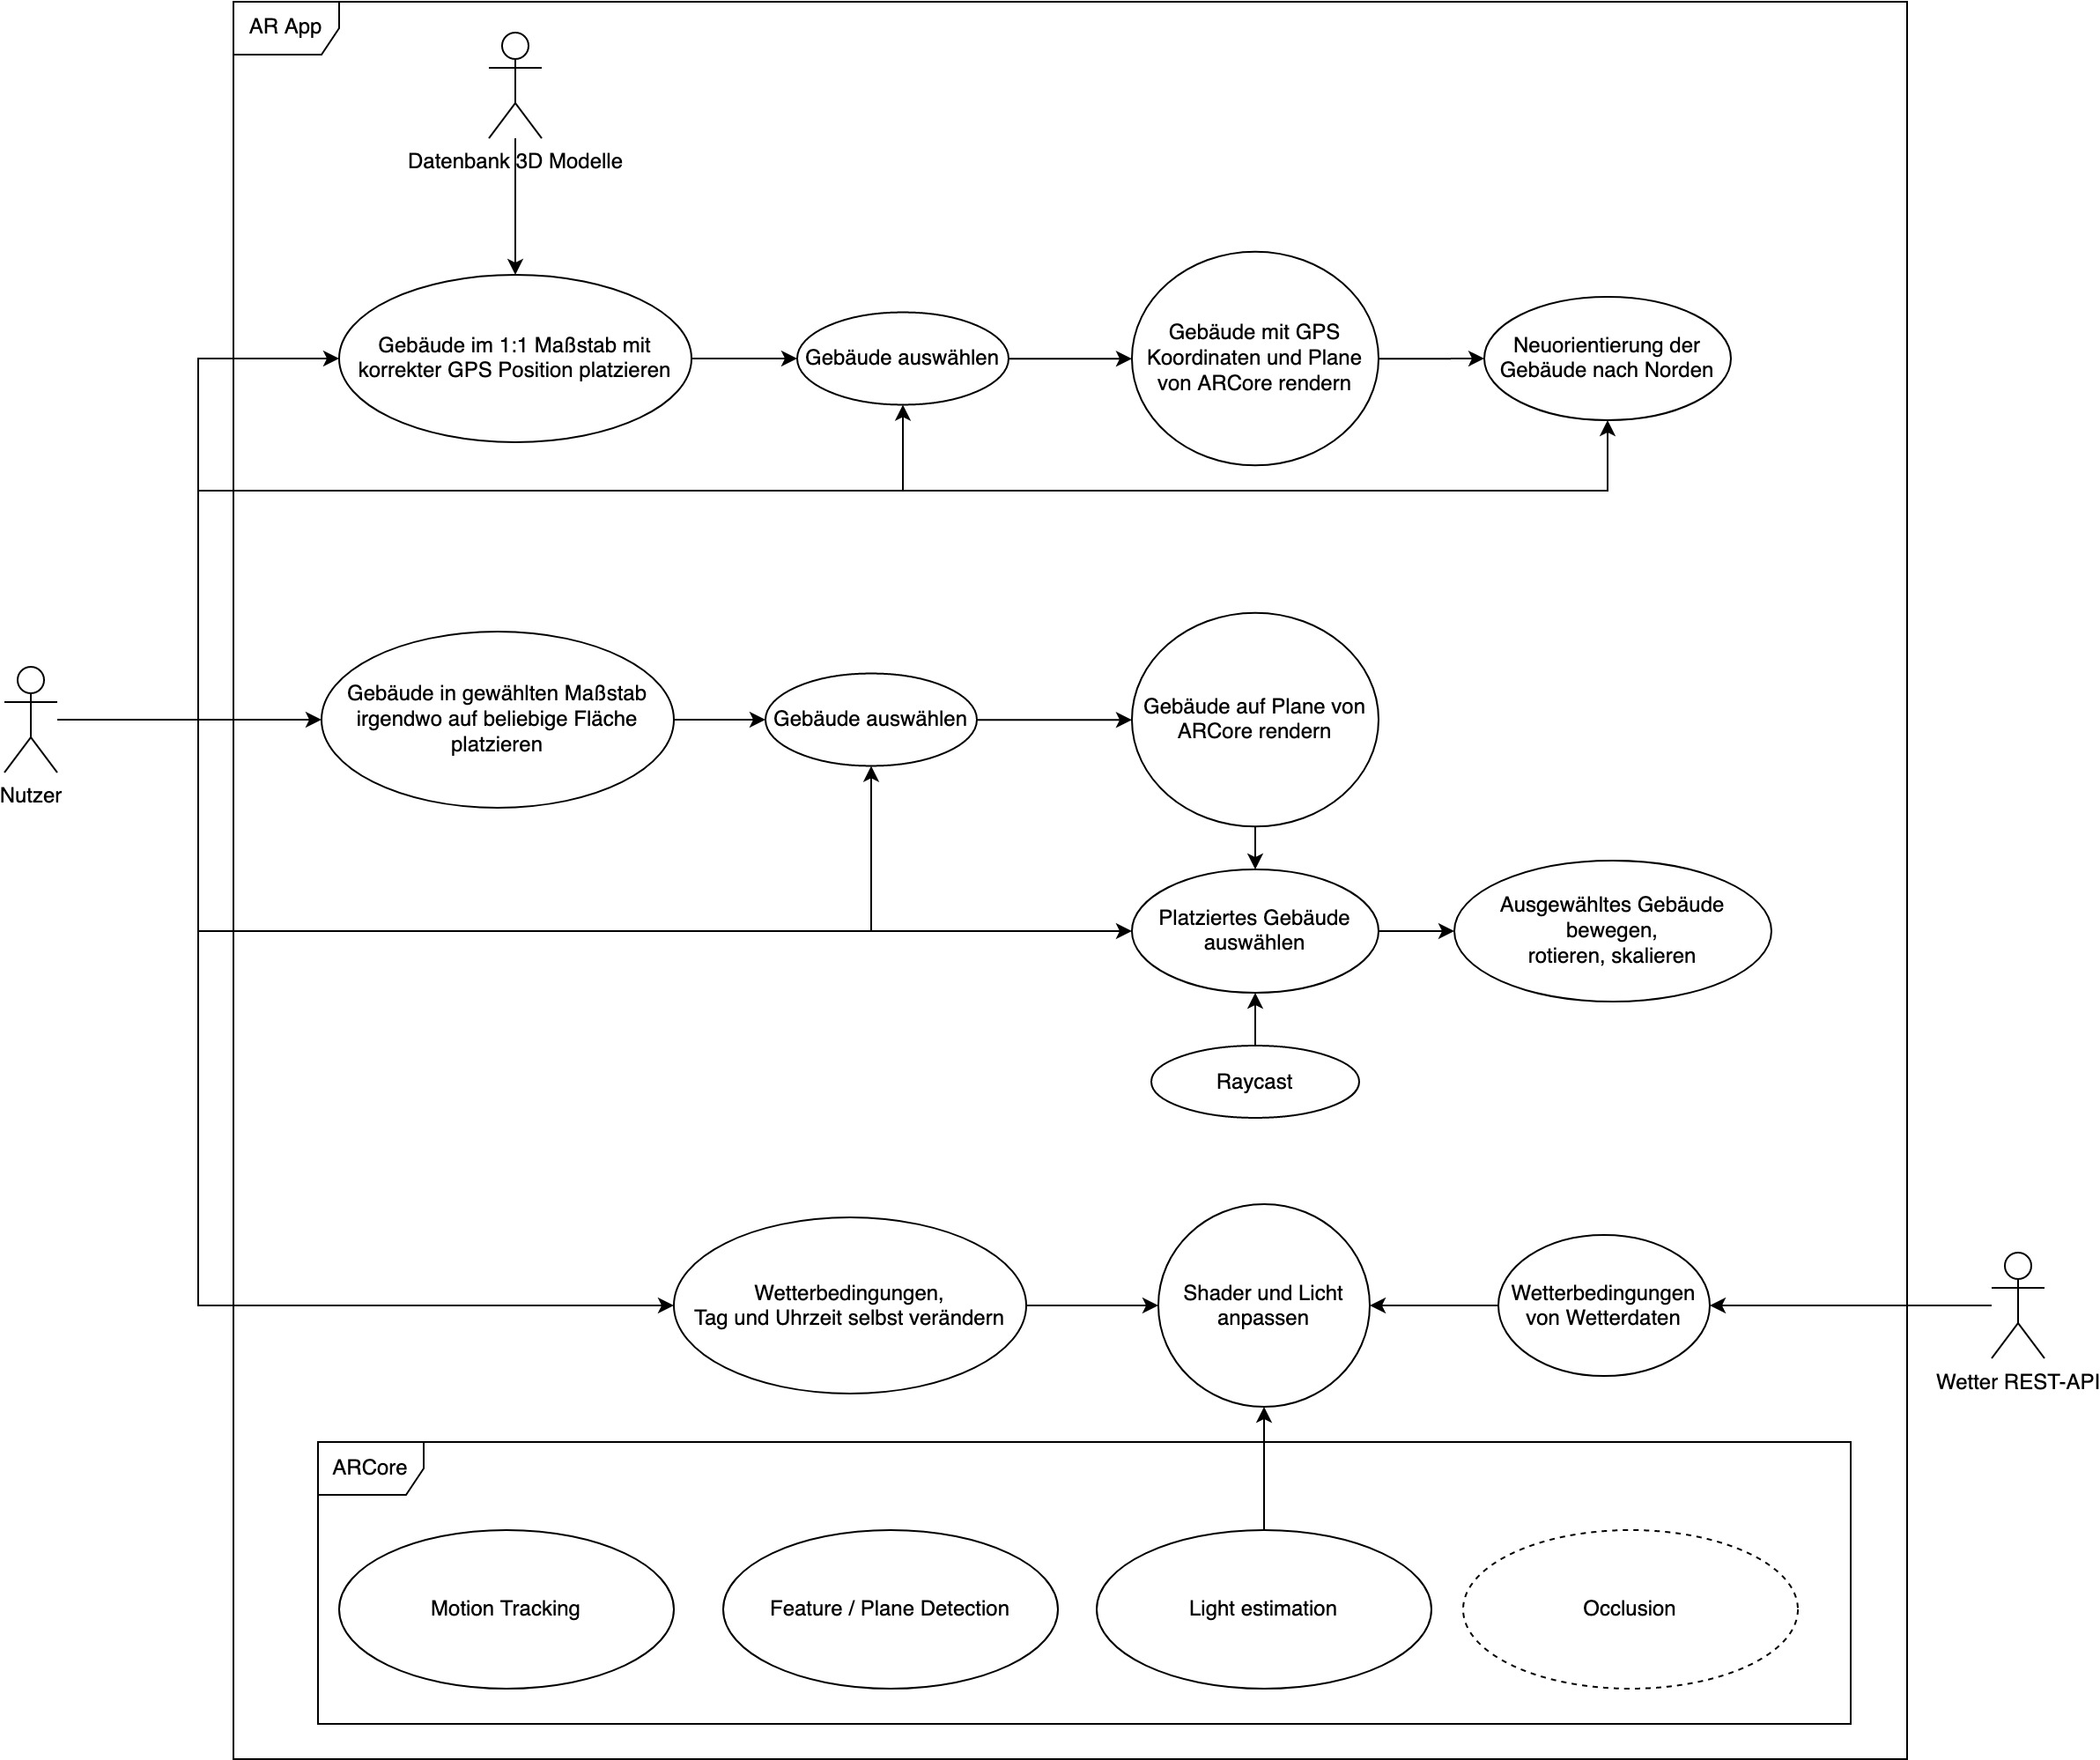
\includegraphics[width=\textwidth]{img/anwendung/UseCaseDiagrammVillingenAR.jpg}
    \caption[Das Use-Case-Diagramm zur Anwendug.]{Das Use-Case-Diagramm zur Anwendug.\protect\footnotemark}
    \label{fig:konzept-use-case-diagramm}
\end{figure}
\footnotetext{Quelle Bild: https://drive.google.com/file/d/1ZhIIEN6V9Jt-uwVcFVNkeFbu1qxbGkaN/view?usp=sharing}

In der Anwendung gibt es drei Akteure: Der Nutzer, die REST-API für die Wetter-Abfrage und eine interne Datenbank mit den Daten zu den Gebäuden. Die interne Datenbank enthält die Informationen zu den Gebäuden, die für die Anwendung benötigt werden. Die Informationen sind:
\begin{itemize}
    \item die 3D Modelle als \textit{Prefab}. Ein Prefab ist ein GameObject in Unity, dass alle Komponenten, Werte und angehängte GameObjects beinhaltet. Sie erlauben dieses GameObject zu speichern und mit den gleichen Informationen wieder zu verwenden\footnote{https://docs.unity3d.com/Manual/Prefabs.html, zuletzt aufgerufen am 13.08.2022},
    \item der Name des Gebäudes, wie z.B. das SABA Hauptgebäude oder das Mannschaftsgebäude,
    \item eine Kurzbeschreibung. Diese wird noch nicht genutzt. Die Idee dazu ist, zusätzlich zum 3D Modell noch eine Kurzbeschreibung des Gebäudes und dessen ehemalige Funktion in AR einzublenden,
    \item die Längen- und Breitengrade für die GPS-Platzierung,
    \item eine Winkelangabe. Diese wird benötigt, um bei einer Ausrichtung nach Norden die Gebäude mit der korrekten Rotation darzustellen,
    \item eine ID-Nummer zur Identifizierung.
\end{itemize}

Die Datenbank wird in Unity mit \texttt{ScriptableObjects}\footnote{https://docs.unity3d.com/Manual/class-ScriptableObject.html, zuletzt aufgerufen am 13.08.2022} realisiert. Das ist ein Datencontainer, indem individuelle Daten gespeichert werden können. Für jedes Objekt wird ein \texttt{BuildingGPS} Scriptable Object erzeugt, indem die jeweiligen Daten gespeichert sind. Die Nutzung der Daten wird in Kapitel \ref*{technische-umsetzung-platzierung-normal} und \ref*{technische-umsetzung-platzierung-gps} behandelt.

Zu Beginn der Anwendung kann der Nutzer in einem Menü sich zwischen zwei Möglichkeiten der Platzierung entscheiden:
\begin{itemize}
    \item das Gebäude wird über GPS Koordinaten platziert,
    \item das Gebäude wird auf einer von ARCore getrackten Flächen platziert.
\end{itemize}

Anschließend wird die jeweilige AR Szene gestartet. An diesem Zeitpunkt wird ARCore gestartet. Die Funktionen wie z.B. das Motion Tracking oder die Plane Detection aktivieren sich. Der Nutzer wählt daraufhin das Gebäude aus, das platziert werden soll. Eine Vorschau des Modells und der Name des Gebäudes werden angezeigt. Dieses Menü ist in Abbildung \ref*{fig:konzept-auswahl-menue} zu sehen. 

\begin{figure}[H]
    \centering
    \subfloat[][]{\includegraphics[width=0.3\linewidth]{img/anwendung/konzept-auswahl-menü.jpg}}%
    \qquad
    \subfloat[][]{\includegraphics[width=0.3\linewidth]{img/anwendung/konzept-auswahl-menü-2.jpg}}%
    \caption{Das Auswahl-Menü. Der Nutzer kann mit dem Burger-Icon das Menü jederzeit öffnen und wieder schließen. Mit den Pfeilen kann zwischen den vorhandenen Gebäuden geschaltet werden.}%
    \label{fig:konzept-auswahl-menue}
\end{figure}

Ist ein Gebäude ausgewählt, ist die Platzierung des Gebäudes möglich. Voraussetzung ist, dass ARCore eine Fläche gefunden hat. Sobald eine Fläche vorhanden ist, wird über Raycast ein Hit-Testing durchgeführt (siehe Kapitel \ref*{technische-umsetzung-arcore-user-interaction}). Ist ein Hit regisitriert, ist eine Fläche für die Platzierung vorhanden. Der Nutzer erhält Feedback über ein Pfeil-Icon, das auf die jeweilige Fläche platziert wird. Dieser hilft dem Nutzer bei der Orientierung und der Platzierung der Objekte.

\subsection{Platzierung auf einer beliebigen Fläche}
Der Pfeil auf dem Boden zeigt an, wo die Position des Gebäude sein wird. Nach der Auswahl des Modells kann der Nutzer über ein Tap auf dem Bildschirm das Gebäude platzieren. Über einen Raycast wird das platzierte Modell erkannt und der Nutzer kann mit einem Button das platzierte Gebäude auswählen. Dieses kann per Drag Gesten über erkannte Flächen verschoben werden. Mit einer Pinch Geste wird das Gebäude skaliert. Über einen Slider wird die Rotation verändert. Nur ausgewählte Gebäude können bewegt, skaliert, rotiert und gelöscht werden. Es ist nur möglich eine Instanz von einem Gebäude zu platzieren.

\subsection{Platzierung über GPS}
Bei der GPS Platzierung wird die aktuelle GPS Position abgefragt. Mit den Längen- und Breitengraden aus der Datenbank werden die Gebäude bezüglich der GPS Position des Smartphones platziert. Damit das Gebäude nicht in der Luft schwebt, wird es auf eine Fläche platziert, die ARCore detektiert hat. Der Nutzer hat hier nicht die Möglichkeit ein Gebäude auszuwählen, da diese Funktion nur vor Ort funktioniert. Der Sinn dieser Funktion ist es, dem Nutzer die Gebäude so zu zeigen, wie sie vor Ort ausgesehen haben. Die Gebäude werden an der jeweiligen Position im Größenverhältnis 1:1 dargestellt.

Der Nutzer hat zusätzlich die Möglichkeit mithilfe des Kompass des Gerätes die Szene nach Norden auszurichten. Damit wird sichergestellt, dass das Gebäude in der korrekten Rotation dargestellt wird. In der Datenbank ist das 3D Modell zusammen mit einer Winkelangabe gespeichert. Diese wird benötigt, um das Gebäude so zu drehen, dass es in die korrekte Richtung zeigt. Die technische Umsetzung wird in Kapitel \ref*{technische-umsetzung-platzierung-gps} behandelt.

\subsection{Licht und Wetterbedingungen ändern}
Die Wetterbedingungen werden beim Start der Anwendung von der REST-API abgefragt. Hierfür wird eine Internetverbindung benötigt. Die Informationen zu Wetter und Tageszeit werden dazu, genutzt das Licht und die Shader der Gebäude anzupassen. Zusätzlich wird die Light estimation Funktion von ARCore genutzt, um die Farbtemperatur und die Helligkeit anzupassen.